\section{FFS}
\label{sec:ffs}
The artifact developed as a result of this degree project is the \glsxtrfull{FFS}. It uses an \gls{OWS} to store the data and behaves as a mountable filesystem for its user. As mentioned in Section~\ref{sec:delim} this is a \mbox{proof-of-concept} prototype of a deniable filesystem using an \gls{OWS} for storage and does \textbf{not} support all of the functionalities that other filesystems do, such as links or access permissions. The reasoning is that these behaviors are not required for a minimally usable filesystem. Additionally, when comparing \gls{FFS} to distributed filesystems, such as Google Drive, many other filesystems do not support functionality such as links.

This section presents the design and implementation details of \gls{FFS}. \Cref{subsec:ffs_impl_overview} presents a general overview of the filesystem and its internal structures. Following, the different caches of the filesystems are presented in~\Cref{subsec:ffs_impl_cache}. The encoding and encryption methods are presented in~\Cref{subsec:file_enc_dec}. \Cref{subsec:ffs_ows} presents Flickr as the target \gls{OWS} used by \gls{FFS} and explains why Twitter could not be used as the \gls{OWS}. \Cref{subsec:file_op} presents the implementation details of each \gls{FUSE} filesystem operation implemented by \gls{FFS}. Finally, \Cref{subsec:ffs_limits} presents the limitations of the filesystem.

\subsection{Design overview}
\label{subsec:ffs_impl_overview}
\gls{FFS} uses images to store all of the filesystem's data, \ie files, directories, and the inode table of the filesystem. These images are uploaded to an \gls{OWS}, such as Flickr, as image posts. As mentioned in~\Cref{sec:ows}, there may be limitations on the size of these posts for certain \glspl{OWS}. To support files larger than these limitations, these files are split into multiple posts, requiring \gls{FFS} to keep track of a list of posts. \Cref{fig:ffs_inode_diag} presents the basic outline of \gls{FFS} and an example of the contents of the filesystem. \gls{FFS} is based on the idea of inode filesystems and uses an inode table to store information about the files and directories in the filesystem. However, instead of an inode pointing to specific blocks in a disk, the inode table of \gls{FFS} keeps track of the IDs of the posts (\ie post ID) on the \gls{OWS} where the file or directory is located. The inode table entry for each file or directory also contains metadata about the entry, such as its size and a Boolean flag indicating whether the entry is a directory.

\begin{figure}[!ht]
	\begin{center}
	  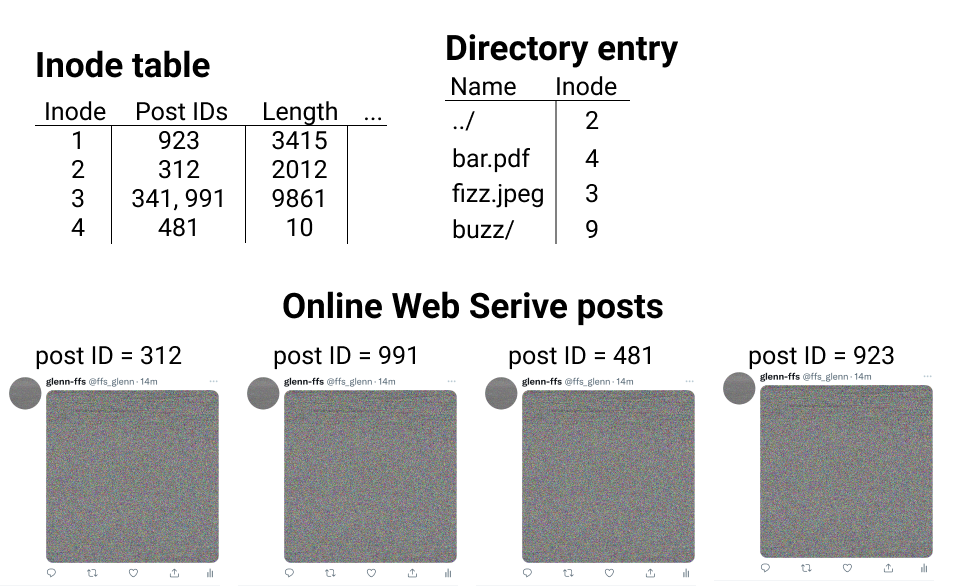
\includegraphics[width=0.99\textwidth]{figures.nosync/ffs_inode_diagram.png}
	\end{center}
	\caption{Basic structure of \gls{FFS} \mbox{inode-based} structure}
	\label{fig:ffs_inode_diag}
\end{figure}
\FloatBarrier
\newpage
\gls{FFS} can be mounted to the local filesystem using \gls{FUSE}, similar to mounting a network drive or a \gls{FTP} server. The mounted \gls{FFS} volume operates similarly to any other drive and can be accessed using, for instance, Mac's Finder or a shell terminal.

The directories and inode table are represented as classes in C++. \Cref{lst:dir_itable_classes} visualizes the main attributes of the \texttt{Directory}, \texttt{InodeTable}, and \texttt{InodeEntry} classes. There can be multiple \texttt{Directory} and \texttt{InodeEntry} objects in the computers' memory and the filesystem, but there will only exist one relevant \texttt{InodeTable} instance. The \texttt{Directory} class is a data structure that stores mappings between filenames and the files' and directories' inode, for all files and directories stored in that directory. The \texttt{InodeEntry} is a data structure that keeps track of a file's or directory's information, such as where the data is stored and its metadata, such as size and creation timestamp. The \texttt{InodeTable} stores a mapping between an inode and the file's \texttt{InodeEntry}. The \texttt{InodeTable} has always at least one entry for the root directory. This entry has a constant inode value of 0 for simplicity to look up the root directory. With the help of the root directory, all the files lower in the directory hierarchy can be found. The inode of all files and directories other than the root directory has a unique inode greater than 0. The \texttt{InodeTable} is always the most recent image saved on the \gls{OWS}, making it easy to find it on the \gls{OWS}. The other images stored on the \gls{OWS} can be images stored in \gls{FFS}, or images posted by the user that does not contain \gls{FFS} data as long as the most recent image saved on the \gls{OWS} is the inode table. The inode table will keep track of which images are stored in the filesystem, and ignore all the other files.

%\chapter[Directory, InodeTable, and InodeEntry class and attributes representation]{Directory, InodeTable, and\\InodeEntry class and attributes\\representation}
%This chapter presents \mbox{pseudo-code} of the different data structures used by \gls{FFS}. 
\Cref{lst:dir_itable_classes} presents \mbox{pseudo-code} of the different data structures used by \gls{FFS}. Each C++ class instance is encoded into a binary representation of the object when it is serialized before being uploaded to the \gls{OWS}. When an object is deserialized, the corresponding C++ class instances are generated \mbox{in-memory}. These serialized representations are described in \Cref{app:binary_rep}.

\Needspace*{39\baselineskip}
%\label{app:inode_dir_code}
\begin{lstlisting}[language=python, caption={Classes representing directories and the inode table in \gls{FFS}}, label=lst:dir_itable_classes,breaklines=true]

# typedef inode_id = uint32_t

# Represents a directory in FFS. Keeps track of the filename and inode of each file
class Directory
	# Map of (filename, inode id) representing the content of the directory
	map<string, inode_id> entries

# Represents an entry in the inode table, representing a file or directory
class InodeEntry
	# The size of the file (not used for directories) 
	uint32_t length

	# True if the entry describes a directory, false if it describes a file
	uint8_t is_dir

	# When the file first was created
	uint64_t time_created
	# When the file was last accessed
	uint64_t time_accessed
	# When the file was last modified
	uint64_t time_modified

	# A list representing the posts of the file or directory. 
	string[] post_ids

# Represents the inode table of the filesystem. The table consists of multiple inode entries
class InodeTable
	# Map of (inode id, inode entry) for each file and directory in the filesystem
	map<inode_t, InodeEntry> entries
\end{lstlisting}

\clearpage

To read the content of a known filename in a directory has three steps using these data structures:
\begin{enumerate}
    \item The \texttt{Directory} object of the directory provides the inode of the given filename.
    
    \item The inode is used to get the \texttt{InodeEntry} from the \texttt{InodeTable}.
    
    \item Using the inode entry, the file can be located.
\end{enumerate}

The location of a file or directory is an ordered list of unique IDs of the image posts on the \gls{OWS}. The data received by downloading these images, decoding them (as described in~\Cref{subsec:file_enc_dec}), and concatenating them, can be read as a file or represented as a \texttt{Directory} object, depending on whether the \texttt{InodeEntry} was marked as a file or a directory. 

As directories only know the filename's inode, the \texttt{Directory} object does not have to be updated (and thus uploaded) when a file or directory in it is edited, for instance when adding data to a file. Only the \texttt{InodeEntry}, and thus the \texttt{InodeTable}, needs to be updated with the new post IDs of the new file or directory. This saves time as every request to the \gls{OWS} takes time. However, if the filename is changed or the file or directory is moved to another location, then the parent directory of the file or directory would have to be updated, and thus its corresponding \texttt{Directory} object has to be updated.

When a new file or directory is created, it is saved in its parent directory with its filename and an inode. This same inode is used in the inode table to keep track of the file's or directory's inode entry. The inode is represented as an unsigned \mbox{32-bit} integer (\ie a \texttt{uint32\_t} as shown in~\Cref{lst:dir_itable_classes}). The inode is calculated by adding one to the currently greatest inode. This means new files and directories will always receive a greater inode value than those currently in the inode table. This naïve approach to inode generation does not take into account that there might be an available inode less than the greatest inode in the inode table (for instance, due to the deletion of a previously created file). However, this inode generation approach is fast and will not be a problem until the integer overflows. As the inode is represented using a \mbox{32-bit} unsigned integer, \gls{FFS} would need to have saved more than four billion files and directories before the inode value would overflow. This scenario is outside the scope of this \mbox{proof-of-concept} filesystem.

As described earlier, \gls{FFS} implements the subset of \gls{FUSE} operations shown in~\Cref{tbl:fs_impl_op}. These operations are those essential for a minimal filesystem\,\cite{kuenningCS135FUSEDocumentation2010}. Operations such as \texttt{chown} provide extended capabilities of the filesystem but are not required for a \mbox{proof-of-concept} filesystem. The functionality of each of the filesystem operations implemented by \gls{FFS} and their implementation details are described in~\Cref{subsec:file_op}. 

% REMOVE FOR PANDOC
\begin{table}[!ht]
	\begin{center}
		\caption{Filesystem operations implementable through the \gls{FUSE} \gls{API}, and whether or not \gls{FFS} implements them}
		\begin{tabular}{| c | c |}
			
			\hline
			\begin{tabular}{@{}c@{}}\textbf{Filesystem operations} \\ \textbf{implemented by FFS}\end{tabular} &
				\begin{tabular}{@{}c@{}}\textbf{Filesystem operations} \\ \textbf{\textit{not} implemented by FFS}\end{tabular} \\
			\hline
			\hline
			\texttt{open} & \texttt{readlink}\\
			\texttt{opendir} & \texttt{symlink}\\
			\texttt{release} & \texttt{link}\\
			\texttt{releasedir} & \texttt{chmod}\\
			\texttt{create} & \texttt{chown}\\
			\texttt{mkdir} & \texttt{fsync}\\
			\texttt{read} & \texttt{fsyncdir}\\
			\texttt{readdir} & \texttt{lock}\\
			\texttt{write} & \texttt{bmap}\\
			\texttt{rename} & \texttt{setxattr}\\
			\texttt{truncate} & \texttt{getxattr}\\
			\texttt{ftruncate} & \texttt{listxatt}\\
			\texttt{unlink} & \texttt{ioctl}\\
			\texttt{rmdir} & \texttt{flush}\\
			\texttt{getattr} & \texttt{poll}\\
			\texttt{fgetattr} & {}\\
			\texttt{statfs} & {}\\
			\texttt{access} & {}\\
			\texttt{utimens} & {}\\
			
			\hline

		\end{tabular}
		\label{tbl:fs_impl_op}
	\end{center}
\end{table}

A file, a \texttt{Directory}, or the \texttt{Inode Table} has to be uploaded to the \gls{OWS} when it is modified to save its current information. As it takes time to make requests to the \gls{OWS}, \gls{FFS} is designed to make as few requests as possible while still saving the required data. Therefore, only the directory or file that is affected by a change is uploaded to the \gls{OWS}. However, the inode table has to be updated with every change of a file or directory as the inode table contains the location of the file or directory.



\subsection{Cache}
\label{subsec:ffs_impl_cache}
\gls{FFS} implements a simple \mbox{in-memory} \gls{LRU} cache for the content downloaded from the \gls{OWS}. The cache consists of two data structures: 
\begin{description}
	\item[Cache Map] a mapping between a post ID and its image data, and
	\item[Cache Queue] a queue keeping track of the cached post IDs.
\end{description}
The cache stores a maximum of 20 image posts. The data stored in the cache is the encrypted image data. To avoid \gls{FFS} using too much memory, the cache is configured so that images greater than \SI{5}{\mega\byte} are not cached. As a result the cache can store a maximum of $20 * \text{\SI[per-mode = symbol]{5}{\mega\byte}} = \text{\SI[per-mode = symbol]{100}{\mega\byte}}$ of encrypted image data. Each time an image is uploaded or downloaded, it is added to the Cache Map with its post ID as the key. The post ID is also added to the beginning of the Cache Queue. If the Cache Queue exceeds 20 elements, the last element of the queue is removed, and the corresponding entry in the Cache Map is erased, thus the entry is fully erased from the cache. The queue ensures that the cache is limited to 20 entries, and by using a \gls{FIFO} queue, the queue ensures that the oldest element in the cache is removed when the cache exceeds its limit. When a file or directory is removed from the filesystem, all its data is also removed from the cache, if it is stored there.

Before a post with a specified post ID is downloaded from the \gls{OWS}, the cache is checked to see if the cache is currently storing this post ID. If so, the stored image is returned. Otherwise, the process continues by downloading the image from the \gls{OWS} and then adding it to the cache (if it is smaller in size than the limit stated above). When the thesis states that a file or directory is downloaded, it is implied that the cache is also checked and the data is possibly returned by the cache instead of requiring a download of the data from the \gls{OWS}.

\gls{FFS} separately caches both the root directory and the inode table. As both of these data structures are used in many of the filesystem operations, it is important that they can be accessed quickly and not be removed from their cache. Their cache entries are updated when the files are uploaded to the \gls{OWS}. They are stored as an instance of an \texttt{InodeTable} object and an instance of a \texttt{Directory} object, respectively.

Additionally, \gls{FFS} separately caches the inode of open files and the inode of the open file's parent directory. The open file's clear text data is also cached in memory if it has been read or written to while it is open. A file is opened with the use of the \texttt{open} or \texttt{create} filesystem operation, as described further in~\Cref{subsec:file_op}. When a file is opened it is associated with a file handle identifier that is used for subsequent filesystem operations to refer to the file rather than using the path to the file in the filesystem. When a user is reading or writing data to a file, multiple \texttt{read} or \texttt{write} file operations might be executed. For instance, when writing a \SI{100}{\byte} file two \texttt{write} operations might be executed:
\needspace{2\baselineskip}
\begin{itemize}
	\item One with \texttt{offset = 0} and with a buffer size of \SI{50}{\byte} bytes, and
	\item One with \texttt{offset = 50} and with a buffer size of \SI{50}{\byte}.
\end{itemize}
The number of \texttt{read} or \texttt{write} operations required to read or write data depends on the amount of data to read or write, and the buffer size used by the file operation which depends on the buffer sizes supported by the filesystem. macFUSE can be mounted with a maximum buffer size of \SI{32}{\mega\byte}\,\cite{fleischerMountOptionsOsxfuse2020}. To save computation time by not having to download the file from the \gls{OWS}, or even decrypt the image data found in \gls{FFS}'s regular cache, \gls{FFS} stores the file's clear text data separately in memory. When a file with a file handle is modified or read, \gls{FFS} checks if the file handle has any cached data associated with it, before checking the regular cache for the post ID. If there is data associated with the file handle, then this data is used for the file operation. If the file operation was a modifying operation, such as a \texttt{write} operation, the new data is associated with the file handle and stored in memory. When the file is closed with a subsequent \texttt{close} file operation, the modified data is encoded, encrypted, and the resulting image file uploaded to the \gls{OWS}. \gls{FFS} does not limit how many files can be open in the filesystem at the same time, nor how much modified data can be associated with a file handle. However, such limits can be imposed by the operating system. If a file in \gls{FFS} is not closed, the associated data is not disassociated with the file handle and is kept in the memory until the filesystem is shut down. Implications of this are discussed in~\Cref{subsec:ffs_limits}.

Furthermore, an additional filesystem cache is provided by the operating system kernel\,\cite{fleischerMountOptionsOsxfuse2020, gowdappaExperiencesFUSEReal2019}. \gls{FFS} can not control the kernel cache other than disabling the cache when the filesystem is mounted. By default, \gls{FFS} does not disable the \gls{UBC} when \gls{FFS} is mounted but the \gls{UBC} can be disabled by the user when mounting \gls{FFS} using \gls{FUSE} command line arguments.
% However, as this operating system provided cache provides faster filesystem operations, it is beneficial for \gls{FFS} to use this. While this could be a problem if another user modifies the state of the filesystem on the \gls{OWS} while \gls{FFS} is mounted, \mbox{multi-user} support is not within the scope of this thesis. The size of the kernel cache has not been found during this research.
% TODO: According to chips url, it can be configured. Not sure though

\subsection{Encoding and decoding objects}
\label{subsec:file_enc_dec}
Entities that \gls{FFS} stores on the \gls{OWS}, encoded as images before being uploaded and when downloaded are decoded. These entities are files, \texttt{Directory} objects, and the \texttt{Inode Table} object. All of these entities are stored on the \gls{OWS} using PNG images with \mbox{16-bit} \gls{RGB} color depth, without an alpha channel. The inode table and the directories are represented as C++ objects in memory during runtime but are serialized into a binary representation before they are encoded into images. The files saved to \gls{FFS} are written into memory in a binary format and encoded into images. All the data encoded into images are encoded similarly, and a detailed description of the binary structures can be found in~\Cref{app:binary_rep}. 

The input to the image encoder is the binary data to encode as an image. A header (\gls{FFS} header) is prepended to the binary data, containing among other things, the size of the data and a timestamp of when the data was encoded. The \gls{FFS} header and the input data are encrypted using authenticated encryption, utilizing \gls{GCM} and \gls{AES}. The key used for the encryption is derived using the \gls{HKDF} function utilizing the \mbox{\gls{SHA}-256} hashing algorithm, along with a random \SI{64}{\byte} salt vector, \mbox{re-generated} every time new data is encrypted. The salt is stored with the cipher to ensure that the decryption algorithm uses the same salt to derive the decryption key. The secret used in the \gls{HKDF} is a password provided by the user. \gls{HKDF} also uses a random \gls{IV}, \mbox{re-generated} every time new data is encrypted. The length of the \gls{IV} is set to 12 bytes. The data resulting from the encryption is the salt, the \gls{IV}, and the encrypted cipher text (including the authentication tag). These three data elements are concatenated into a string of bytes. This string of bytes is referred to as the \gls{CED}.

As described in~\Cref{sec:data_storage}, the dimensions of an \gls{FFS} image are based on the number of bytes stored. The stored data is the CED, prepended with the Length of the \gls{CED} (\ie the \gls{LCED}) using four bytes. For an image of $X = \ceil{\frac{4 + LCED}{6}}$ pixels\footnote{$\ceil{x}$ is the \texttt{ceil} function, rounding $x$ up to the closest integer}, \gls{FFS} will set the width $w$ of the image as $w = \ceil{\sqrt{X}}$. The height $h$ of the image is set as $h = \ceil{\frac{X}{w}}$. This will require $(w * h) - X$ filler bytes and will create an image with a similar height and width. For certain values of $X$, $h$ will be equal to $w$. For other values of $X$, $h = w-1$. The resulting data encoded as pixels in the image is, in order:
\needspace{4\baselineskip}
\begin{itemize}
	\item four bytes representing the \gls{LCED},
	\item the \gls{CED} data, and
	\item random filler bytes.
\end{itemize}

The data consisting of the \gls{LCED}, CED, and filler bytes are encoded into \gls{PCD} for a PNG with 16 \gls{RGB} bit color depth using the Magick++ library. The result is an image with a high probability of what looks like random colors for each pixel. This is because most pixels are encrypted data and therefore the bytes representing this data are seemingly random colors.

To decode an \gls{FFS} image, the decoder first interprets the four first bytes as the \gls{LCED}. The salt and \gls{IV} are retrieved from the \gls{CED} as they are of known length. The decryption key is derived using the \gls{IV} and salt and results in the same key as the encryption key because \gls{AES} is a symmetric cipher algorithm. The remaining bytes of the \gls{CED} ($\gls{LCED} - len(IV) - len(salt)$ bytes) are decrypted using the decryption key. The decrypted data consists of the \gls{FFS} header concatenated with the original stored data. The \gls{FFS} header is asserted to be in the correct format before the original binary data is returned from the decryption function. Figure~\ref{fig:file_enc_dec} visualizes the encoder and decoder for all data saved in \gls{FFS}.

\begin{figure}[!ht]
	\begin{center}
	  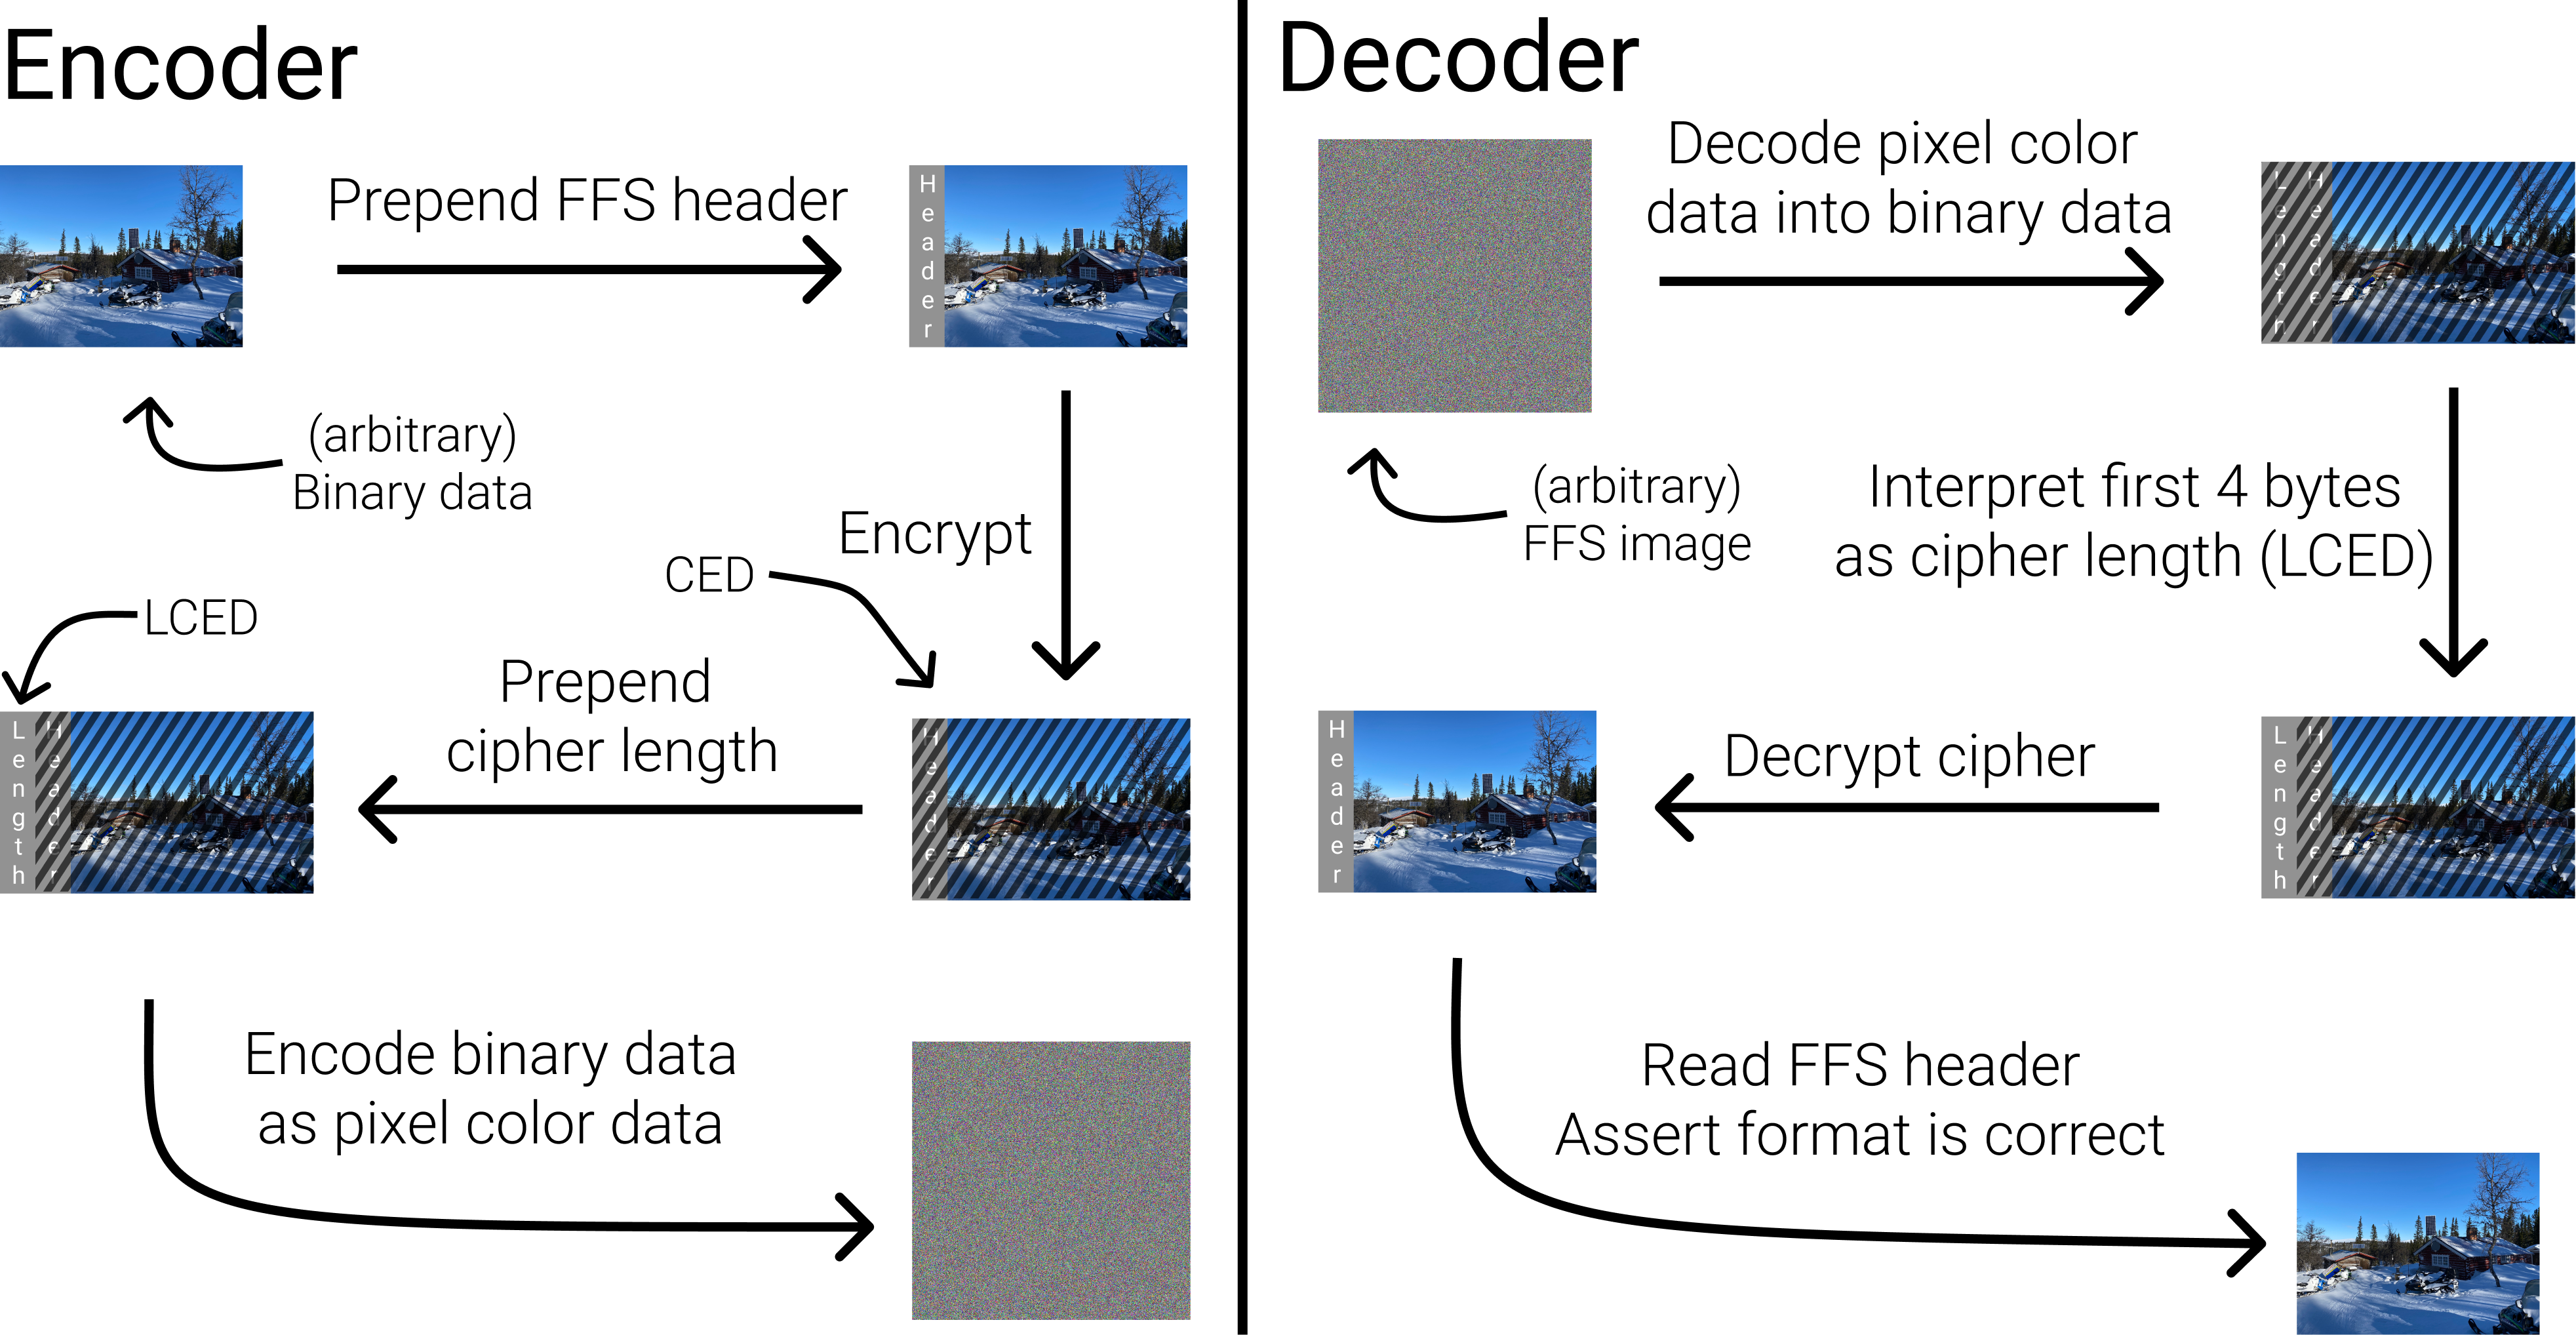
\includegraphics[width=1.0\textwidth]{figures.nosync/encoder_decoder.png}
	\end{center}
	\caption[Simple visualization of the encoder and decoder of \gls{FFS}]{Simple visualization of the encoder and decoder of \gls{FFS}. The input to the encoder is the binary data to store in \gls{FFS}, \eg a file, and the output is the \gls{FFS} image to upload to the \gls{OWS}. The input to the decoder is an \gls{FFS} image, and the output is the binary data stored on \gls{FFS}, \eg a file.}
	\label{fig:file_enc_dec}
\end{figure}

The encryption and decryption methods used are \mbox{state-of-the-art} solutions as defined and implemented by Crypto++\,\cite{CryptoLibraryFree}. Crypto++ is a \mbox{widely-used} and \mbox{well-maintained} C++ library for cryptography, and as of writing has no reported CVE security vulnerabilities for the functionality used by \gls{FFS}\,\cite{CryptoppSecurityVulnerabilities}.

An \gls{FFS} image has an upper size limit, defined by the \gls{OWS} used. If the data to be stored in \gls{FFS}, such as a file, exceeds this limit, it is split into multiple data arrays of sizes less than this limit. Each data array is encrypted and encoded as images independently of each other, and will be encrypted using different salts and \gls{IV}s. However. the inode table stores the different post IDs in the order they were encoded. While files and directories stored in \gls{FFS} can be separated into multiple images, the inode table is limited to a single image for simplicity when interacting with the \gls{OWS}. This introduces a size limit for the inode table, thus limiting the filesystem. More details about the limits of \gls{FFS} are found in~\Cref{subsec:ffs_limits}.

\subsection{Online web services}
\label{subsec:ffs_ows}
As \gls{FFS} is a \mbox{proof-of-concept} filesystem, it only uses one \gls{OWS} as its storage medium. However, for a production filesystem, using multiple \glspl{OWS} could be beneficial. This would enable features such as redundancy by using replication over multiple \glspl{OWS}, such redundancy could be useful in case one \gls{OWS} would stop working or be inaccessible.

The initial intention of \gls{FFS} was to use Twitter as the \gls{OWS}. Initial research for the thesis found that it was possible to upload a file and download the same file without any data loss. However, it was later found that this was not a reliable conclusion. Some images uploaded to Twitter were converted to another image format when they were stored by Twitter, which meant that the decoder could not decode the data as it expected another image format. Other images were compressed or \mbox{re-coded} which led to data loss when downloading the image. As the decoder of \gls{FFS} images relies on a specific binary representation within the image, this meant that the images could not be decoded into the previously uploaded data. Twitter has previously publicly announced changes to the way they store images\,\cite{nolanobrienUpcomingChangesPNG2018} and even suggested workarounds\,\cite{nolanobrienFeedbackUpcomingChanges2019} for users who are concerned about the potential data loss. However, during research for the thesis, it was concluded that the workarounds mentioned in \cite{nolanobrienFeedbackUpcomingChanges2019} no longer work on Twitter. For instance, some PNG images less than 900x900px uploaded to Twitter could not be downloaded as the same image, which contradicts the workaround mentioned in \cite{nolanobrienFeedbackUpcomingChanges2019} by the Twitter employee. Further changes may have been made to the data management of images on Twitter since the initial research for the thesis; however, an official announcement has not been found.

Flickr saves the original version of the uploaded image, and thus it can be used to download the same image as was uploaded. This means that data encoded into an \mbox{\gls{FFS}-encoded} image can be uploaded, downloaded, and decoded into the same data as before. While they do not assure that they will always support original images, they have not indicated this would change. Therefore, Flickr can be used at this moment for \gls{FFS}. Therefore, a \mbox{free-tier} Flickr account was used for \gls{FFS}. Restrictions can be set on the Flickr account to enable or disable unauthenticated Flickr visitors from downloading the originally uploaded image. The advantage of enabling unauthenticated Flickr visitors to download the images is that the user can read the content of \gls{FFS} even if they do not authenticate with Flickr, and the data can be shared with others using only the password used for encrypting the data in \gls{FFS}. The disadvantage is that adversaries can also download these images and potentially gain information about the data stored in \gls{FFS} even if they do not have the encryption password for \gls{FFS}. However, even by restricting downloading of the original images, adversaries can still access the original images, for instance, if Flickr provides them. Therefore, the Flickr account was set to allow unauthenticated visitors of Flickr to download the original versions of the images.

Flickr provides an extensive free REST \gls{API} for \mbox{non-commercial} use. A user can create applications and generate access tokens for the application. These application tokens are later used to request tokens from users who authenticate using Flickr's web interface and allow the application to make requests on behalf of the user. The application will then receive access tokens for the user, which are used to authenticate with the \gls{API} for those \gls{API} calls that require authentication.

Flickr provides the ability to search for all the images posted by a user and to sort these results by the time of posting. In \gls{FFS}, every time an image is uploaded to Flickr, it is due to some modification in the filesystem, for instance, a write operation to a file or a creation of a new directory. For every modification in the filesystem, the inode table will have to be updated. Therefore, we can ensure that the inode table is always the most recently uploaded image to Flickr by configuring \gls{FFS} to upload all other images first, for instance, the newly written file. This provides \gls{FFS} with a simple way of querying the inode table from Flickr - by simply requesting the most recently uploaded image on the Flickr account.

While the Flickr \gls{API} is extensive in its functionality, \gls{FFS} only uses a few of the provided capabilities; specifically \gls{FFS} uses:
\needspace{6\baselineskip}
\begin{itemize}
	\item Upload an image and return the post ID;
	\item Query the most recent image by a user, and return the URL and post ID of the original uploaded image;
	\item Get the URL to the original uploaded image given a post ID;
	\item Remove an image given a post ID; and
	\item Get the image data of the image given its URL.
\end{itemize}

For instance, to download the original image given a post ID, two requests are required:
\needspace{3\baselineskip}
\begin{enumerate}
	\item Get the URL to the original uploaded image given a post ID and
	\item Get the image data of the image given its URL.
\end{enumerate}
\needspace{12\baselineskip}
For benchmarking purposes, a fake variant of \gls{FFS}, \gls{FFFS}, has also been developed. \gls{FFFS} uses a \gls{FOWS}, which stores the data on the local \gls{APFS} filesystem. \gls{FOWS} is used by \gls{FFFS} just as Flickr is used by \gls{FFS}, by storing encoded images on it. By storing the images on the local filesystem, the filesystem operation's duration is shorter as the local filesystem operations are generally faster than network requests. This allows us to analyze the theoretical performance limit of \gls{FFS}, and how it would perform if the \gls{OWS} used had very low latency and the network connection to the \gls{OWS} had very high bandwidth and low delay. By analyzing \gls{FFFS}, one can also estimate how much of the filesystem's operation time is affected by the response time of the network requests. The time $T$ of an \gls{FFS} filesystem operation can be modeled as:
$$
	T = t_\text{ffs} + t_\text{ows}
$$
where $t_\text{ffs}$ is the time that \gls{FFS} takes, for example, for a read operation on a file associated with a file handle this involves:
\needspace{5\baselineskip}
\begin{itemize}
	\item finding the file in the inode table,
	\item decoding and decrypting the image data,
	\item reading the specified amount of data, and,
	\item to output the data.
\end{itemize}
This time will be approximately constant for the same request for the same file size. However, memory cache misses/hits and process scheduling, among other factors, can vary the value of $t_\text{ffs}$. In contrast, $t_\text{ows}$ is the total time required to complete all requests to the \gls{OWS} for a filesystem operation. For instance, for a similar read operation as above, this consists of:
\needspace{4\baselineskip}
\begin{itemize}
	\item downloading all the directories in the file path,
	\item querying the Flickr \gls{API} for the URL pointing to the most recently uploaded image, and
	\item downloading the images representing the file to be decoded and read subsequently (as part of $t_\text{ffs}$).
\end{itemize}

Depending on the \gls{OWS}, the latency and bandwidth of the internet connection between the user's machine and the \gls{OWS}'s server can vary a lot. Repeated requests to the same \gls{OWS} can also differ due to, for instance, server load balancing and a difference in the number of requests from other users at the time of the requests. Furthermore, the request could be serviced by a cache hit in the \gls{FFS} cache. However, for a \gls{FOWS}, $t_\text{ows}$ can be replaced by $t_\text{fows}$, which will have approximately constant values for repeated operations because the local filesystem is unaffected by the network connection or the current traffic by other users of the shared \gls{OWS}. While running the benchmarking tool, the local filesystem requests by other applications on the machine should be minimized by not using other applications on the machine and thus ensuring that filesystem requests by the \gls{FOWS} can be consistently handled by the operating system. However, $t_\text{fows}$ is affected by, among other things, the underlying storage device of the local filesystem, process scheduling, and \gls{FFS} cache hits/misses, which can still affect the value of $t_\text{fows}$.

Due to limitations in the \texttt{Flickcurl} library used for uploading images to Flickr, the image to be uploaded to Flickr first has to be saved to the local filesystem. \texttt{Flickcurl} reads the image from the disk before uploading it. Therefore, \gls{FFS} saves a temporary file on the local filesystem when data is uploaded to Flickr. This temporary file is stored in the \texttt{/tmp} directory of the local filesystem and is removed by \gls{FFS} immediately after the file has been uploaded. However, it is uncertain that the operating system removes or overwrites the file data on the storage device, and thus there are ways to recover the deleted data by, for instance, adversaries\,\cite{llcsysdevlaboratoriesHowRecoverData2022,cedricAPFSDataRecovery2022,santosHowRecoverData2021}. Although, these methods require you to decrypt the \gls{APFS} volume, requiring the decryption password. Without this password, the data cannot be recovered. Even with the decryption password, it is not certain that the data is recoverable. If an adversary obtains proof that an \gls{FFS} image has been present in the \texttt{/tmp} directory, they could conclude that \gls{FFS} has been used to store data, reducing the deniability of the filesystem.

\subsection{Implemented filesystem operations}
\label{subsec:file_op}
This section gives a detailed description of all the \gls{FUSE} operations implemented by \gls{FFS} and how they are implemented by \gls{FFS}. Further explanations about the intended functionality of the operations can be found in \citeauthor{kuenningCS135FUSEDocumentation2010}'s report\,\cite{kuenningCS135FUSEDocumentation2010}. 

The path of a file is sometimes provided for the filesystem operation and traversed by \gls{FFS} to determine the requested location. An example path is \texttt{/foo/bar/buz.txt} or \texttt{/foo/bar/baz/}. A path is traversed with the \mbox{pseudo-code} shown in Listing~\ref{lst:traverse_path}.

\begin{lstlisting}[language=python, caption={Pseudocode of traversing a given path, returning the \texttt{Directory} and the filename}, label=lst:traverse_path,breaklines=true, basicstyle=\footnotesize, float]
# Traverse a given path and return the parent directory object
#  and filename of the path
traverse_path(path) -> (Directory, string):
	# Fetches inode table from the cache
	inode_table := get_inode_table()
	
	split_path := path.split("/")
	# The filename could be either the name of a file 
	#  or the name of a directory
	filename := split_path.last
	dirs := split_path.remove_last()

	# Get the root dir from the cache
	curr_dir = cache.get_root_dir()

	# While there are still directories to traverse,
	#  get the next directory in the list from the 
	# current directory
	while(!dirs.empty())
		dir_name := dirs.pop_first()
		inode := curr_dir.inode_of(filename=dir_name)
		inode_entry = inode_table.entry_of(inode=inode)
		# Download the image posts defined by the 
		#  post IDs in the inode entry
		curr_dir = download_as_dir(inode_entry)
	
	return (curr_dir, filename)

\end{lstlisting}

When traversing a path, \gls{FFS} has to fetch all parent directories in the hierarchy. The file or directory with the filename is not fetched while traversing the path, as it might not be necessary for the operation. All operations that rely on the path of a file or directory have to download all parent directories of the path. However, the directories in the path could be cached and, therefore, not need to be downloaded from the \gls{OWS}. Furthermore, the \texttt{open}, \texttt{opendir}, and \texttt{create} operations associate a file handle with a file or directory. This enables subsequent filesystem operations to use the file handle instead of traversing the string path. This saves time because the path traversing only occurs once for potentially multiple filesystem operations, and the result is saved in the filesystem state.

After every operation that modifies the inode table, the inode table is uploaded to the \gls{OWS} and cached. Therefore, it is assumed that the inode table is always up to date in memory \textbf{and} on the \gls{OWS}. This will be true as long as there are not multiple \gls{FFS} instances working with the same \gls{OWS} account simultaneously. This multiuse scenario has undefined behavior as there is no locking implemented for \gls{FFS}.

All filesystem operations are synchronous unless specified. Further, \gls{FUSE} is running in \mbox{single-thread} mode meaning that a filesystem operation call \textit{must} complete before another can begin. This helps limit the risk of data races as two processes cannot call different operations that, for instance, modify the inode table at the same time.

\subsubsection{open}
Given a path to a file, this file is associated with a file handle. This file handle can be used in subsequent operations to avoid traversing the file path multiple times. The file is not downloaded from the \gls{OWS}; only the parent directories are downloaded during the path traversal, as explained above. An \texttt{open} call must, eventually, be followed by a \texttt{release} call. Although, multiple file operations can occur between these two calls.

\subsubsection{create}
The create operation creates an empty file in the filesystem given a path and associates a file handle with this new file, similar to \texttt{open}. The empty file will \textit{not} be uploaded to the \gls{OWS} as it has no data associated with it. A new entry is added to the parent directory with the filename and the generated inode, and the parent directory is updated in the \gls{OWS}. The new posts representing the parent directory in the \gls{OWS} are associated with the inode entry of the parent directory in the inode table, and the old posts are deleted from the \gls{OWS}. A new inode entry is also created in the inode table, representing the new, empty, file. The inode table is updated in the \gls{OWS}, and the old inode table is removed.

\subsubsection{release}
Given a file handle, the release operation closes the file in the filesystem, disassociating the file handle from the file. The current states of the file and the inode table are saved to the \gls{OWS}, and the previous versions of the file and inode table are deleted from the \gls{OWS}. Subsequent operations on the file will require path traversing as the previous file handle can no longer be used.

Each file must have a file handle associated with it before \texttt{release} is called. This requires a preceding \texttt{open} or \texttt{create} call for the file.

\subsubsection{opendir}
Given a path to a directory, the directory is associated with a file handle. This file handle is used in subsequent operations to avoid traversing the file path multiple times. The directory is not downloaded from the \gls{OWS}; only the parent directories are downloaded during the path traversal, as explained above. An \texttt{opendir} call must, eventually, be followed by a \texttt{releasedir} call. Although, multiple other operations can occur between these events.

\subsubsection{releasedir}
Given a file handle, the releasedir operation closes the directory in the filesystem, disassociating the file handle from the directory. The current states of the directory and the inode table are saved to the \gls{OWS}, and the previous versions of the directory and inode table are deleted from the \gls{OWS}. Subsequent operations on the directory will require path traversal as the previous file handle can no longer be used.

Each directory must have a file handle associated with it before \texttt{releasedir} is called. This requires a preceding \texttt{opendir} call.

\subsubsection{mkdir}
The mkdir operation creates an empty directory in the filesystem given a path. The directory is not uploaded to the \gls{OWS} as it has no data associated with it. The parent directory is modified and updated in the \gls{OWS}, and the old versions of the parent directory are deleted from the \gls{OWS}. The parent directory entry in the inode table is modified with the new posts, and a new entry is created for the new directory. The inode table is updated in the \gls{OWS}, and the old version of the table is removed from the \gls{OWS}.

Unlike \texttt{create} for files, this operation does not associate a file handle with the directory.

\subsubsection{read}
This operation reads $s$ bytes into a data buffer $a$, starting at the provided offset $o$, from an open file utilizing the provided file handle. If the file has not been read or written to since it was opened, the full file is downloaded and read into memory, even if just a small part of the file is requested. The file data is also cached and the cached data is associated with its file handle so that subsequent requests for the same file while it is open are faster. If the file has been read or written to since it was opened, the file data is accessed from the cache using the file handle.

\subsubsection{readdir}
This operation reads the filenames inside the directory specified by a file handle. The result includes all filenames in the directory and the special \texttt{"."} and \texttt{".."} directories.

\subsubsection{write}
The write operation writes $s$ bytes from a data buffer $a$, starting at the provided offset $o$, to the existing and open file utilizing the provided file handle. All the data of the current file is read into memory. Starting from the offset, the new data from $a$ overwrites the current data of the file, until $s$ bytes have been written. If $o + s$ is greater than the file's size, the file size is set to $o + s$. If $o + s$ is less than the file's size, the data from position $o + s$ and forward remains the same, and the file size is not modified. See~\Cref{fig:write_flow} for a visualization of the result of a \texttt{write} operation given different offsets. The parent directory does not have to be modified. 

The file and inode table are not updated on the \gls{OWS}, this occurs instead in the subsequent \texttt{release} call. However, the newly written data is associated with the file handle so that subsequent filesystem calls use this new file data.

\begin{figure}[!ht]
	\begin{center}
	  
\includegraphics[width=0.9\textwidth]{figures.nosync/write_flow.png}
	\end{center}
	\caption{Visualization of how the write operation handles different offsets.}
	\label{fig:write_flow}
\end{figure}
\FloatBarrier

\subsubsection{rename}
This operation renames a file or directory to a new path. Both the old path and the new path have to be traversed to locate the parent directories and the file or directory to rename. The file or directory entry in the old parent directory is removed, and the old parent directory is updated to the \gls{OWS}. A new entry is created in the new parent directory with the new filename. The new parent directory is updated to the \gls{OWS}. The inode entry of the renamed file or directory does not have to be modified. However, as both the old parent directories and the new parent directory are updated in the \gls{OWS}, their inode entries need to be updated with the new posts. The inode table is updated to the \gls{OWS} and the old table is removed from the \gls{OWS}. The old posts associated with the old parent directory and the new parent directory are removed from the \gls{OWS}.

The new path could be in the same directory as the file or directory currently is in. This will not affect the process mentioned above; however, the path will only have to be traversed once, and the parent directory will only be removed and updated once. If the new path is the path of an existing file, the existing file is removed from the filesystem and the \gls{OWS}.

\subsubsection{truncate}
This operation truncates or extends the file in the given path, to the provided size $s$. The full current file is downloaded into memory. The data of the current file is written to a new buffer until either the file is fully written, or until $s$ bytes have been written. If the current file's size is smaller than $s$, the remaining bytes are written as the NULL character. The new file data is uploaded to the \gls{OWS}, and the old data is removed from the \gls{OWS}. The inode table entry is updated with the new posts and uploaded to the \gls{OWS}. The old inode table is removed from the \gls{OWS}.

\subsubsection{ftruncate}
This operation is similar to \texttt{truncate}, but is called from a user context which means it has a file handle associated with it. The operation truncates or extends the file with the given file handle to the provided integer $s$. The full current file is read into memory, either from the \gls{OWS} or from the cache. The data of the current file is written to a new buffer until either the file is fully written or until $s$ bytes have been written. If the current file's size is smaller than $s$, the remaining bytes are written as the NULL character.

The file and inode table are not updated to the \gls{OWS}, this occurs instead in the subsequent \texttt{release} call. However, the data is associated with the file handle so that subsequent filesystem calls use this new file data.

\subsubsection{unlink}
This operation removes a file given the file path. The file is removed from the parent directory, and the parent directory is updated to the \gls{OWS}. The old parent directory data is removed on the \gls{OWS}. The removed file's entry in the inode table is also removed, and the inode table updates the entry for the parent directory with its new posts. The inode table is then updated on the \gls{OWS} and the old inode table is removed on the \gls{OWS}. Finally, the data of the removed file is removed from the \gls{OWS}. The last step is not necessary for a working filesystem; however, to save space on the \gls{OWS}, this is done. If the \gls{OWS} permits unlimited images and unlimited total storage, this step could be omitted to save time.

\subsubsection{rmdir}
Similar to \texttt{unlink}, this operation removes the directory at the given path. The directory and all its subdirectories are traversed, and the post IDs of these files and directories are recorded for deletion later. Following this, the entry of the removed directory is removed from the parent directory. The inode entry for the removed directory is removed. The parent directory is updated to the \gls{OWS}, and the inode table is updated with the new posts of the parent directory. Following this, the inode table is updated to the \gls{OWS}. The old parent directory and the old inode table are removed from the \gls{OWS}.

The operation also starts a new thread, where all the posts of files and subdirectories inside the removed directory, are removed from the \gls{OWS}. They are removed to save space on the \gls{OWS}, and a separate thread is used to minimize the delay for subsequent file operations. There is no data race involved as the \gls{API} is \mbox{thread-safe}, and the posts are no longer associated with any data structures in the main thread and thus could not be accessed there. This also means that this thread can be run with a lower priority.

\subsubsection{getattr}
This operation returns attributes about a file or directory given a path. This includes permissions, the number of entries (if the provided path points to a directory), timestamps of creation, timestamps of last access, and timestamps of last modification. However, as mentioned previously, \gls{FFS} does not implement all of these features, such as permissions. Instead of keeping track of a file's or directory's permissions, all calls to a valid path will return full read, write, and execute permissions for everyone. However, the timestamps are stored in the inode table of \gls{FFS}. The file or directory pointed to by the path does not need to be downloaded, all the metadata that \gls{FFS} stores is accessible through the inode entry in the inode table, and the inode table is always cached.

\subsubsection{fgetattr}
This operation is similar to \texttt{getattr} but is called from a user program context meaning that the file has a file handle associated with it. Other than skipping the path traversal step, this operation returns the equivalent information as \texttt{getattr}.

\subsubsection{statfs}
This operation returns metadata information about \gls{FFS}. This includes, among other things, the maximum filename size and the filesystem ID. This operation has a short execution time as it does not have to download or upload any files. The only variable information is read from the inode table that is cached in memory and thus does not have to be downloaded from the \gls{OWS}.

\subsubsection{access}
This operation, given a path, returns whether or not the path can be accessed. As long as the path is valid, this always returns true.

\subsubsection{utimens}
This operation, provided new timestamps, updates the last access timestamp, the last modified timestamp, or both, of the file or directory at the given path. The file or directory does not have to be downloaded. However, the inode entry for the file's or directory's inode is updated with the new timestamps if they are newer than the previous timestamps but not greater than the current time since epoch. The new state of the inode table is updated to the \gls{OWS}, and the old version is removed from the \gls{OWS}.

\subsection{FFS limitations}
\label{subsec:ffs_limits}
\gls{FFS} has numerous limitations due to both implementation decisions and \gls{OWS} limits. As Flickr allows a \mbox{free-tier} user account to store up to \num{1000} images of up to \SI{200}{\mega\byte} per image, this allows storage of up to \SI{200}{\giga\byte} of images per account on Flickr. However, as the inode table is required to be stored on the filesystem, a maximum of 999 images can be used to save file and directory data. This limits the filesystem to a maximum of 999 files and directories when utilizing one \mbox{free-tier} account on Flickr, which also limits the maximum storage of file- and directory images to \SI{199.8}{\giga\byte}.

While Flicker supports each image being up to \SI{200}{\mega\byte}, it is not possible to use the full \SI{200}{\mega\byte} to store the file or directory data as each image includes, among other things, a PNG header, other PNG attributes, and the \gls{CED} which in total is of greater size than the unencrypted data. To ensure that the \gls{PCD} along with the PNG header and other PNG attributes do not exceed the limit of \SI{200}{\mega\byte}, \gls{FFS} limits the \gls{PCD} size to allow at least \SI{10}{\mega\byte} for the PNG header and other PNG attributes, meaning that the \gls{PCD} can be a maximum of \SI{190}{\mega\byte}. The cryptographic variables \gls{IV}, salt, and the authentication tag are stored in the \gls{CED} using 12, 16, and 64 bytes respectively, for a total of 92 bytes. The size limit means that these 92 bytes, along with the encrypted cipher text, cannot exceed \SI{190}{\mega\byte}, meaning that the encrypted cipher text cannot exceed \num{190000000} - 92 = \num{189999908} bytes. Moreover, as \gls{AES} is a block cipher and produces cipher blocks of 16 bytes, the resulting cipher text must be divisible by 16. The largest encrypted cipher text that \gls{FFS} allows is therefore $\floor{\frac{\num{189999906}}{16}}*16 = \num{189999904}$ bytes\footnote{$\floor{x}$ is the \texttt{floor} function, rounding $x$ down to the closest integer}. Due to plain text padding, the unencrypted plain text can be a maximum of one byte less than this value\,\cite{z.z.coderAnswerSizeData2010}, meaning that the plain text can be a maximum of \SI{189999903}{\byte}. For simplicity, this is rounded down to \SI{189}{\mega\byte}, leaving almost \SI{11}{\mega\byte} in total for the PNG header and other PNG attributes. Therefore, \SI{189}{\mega\byte} is set as the maximum amount of data \gls{FFS} will store per image. Data greater than \SI{189}{\mega\byte} in size is split into multiple encoded images. For instance, a file of \SI{200}{\mega\byte} will be stored as \SI{189}{\mega\byte} in one image, and \SI{11}{\mega\byte} in another. 

With \SI{189}{\mega\byte} of usable data per image, \gls{FFS} has a maximum storage capacity of \SI{188.811}{\giga\byte} using 999 files and directories on one \mbox{free-tier} account on Flickr. Each file with data requires at least one image, thus there can be a maximum of 998 \mbox{non-empty} files and directories in the filesystem, excluding the root directory. However, there could also be just one single entry of \SI{188.811}{\giga\byte} stored in the filesystem, which would represent the root directory.

The inode table keeps the information about empty files and directories even though they store no data on the \gls{OWS}. As described earlier, the inode of a file or directory is an unsigned \mbox{32-bit} integer, thus the inode table could theoretically store more than four billion files and directories. However, due to the constraints mentioned above, most of these files and directories would have to be empty as Flickr limits the number of images stored. An empty file requires \SI{37}{\byte} in the inode table, consisting of the inode, length, and other variables that must exist for an inode entry. As the inode table is limited to one single image on the \gls{OWS}, the inode table is limited to a maximum size of \SI{189}{\mega\byte}. Further, the size of the inode table is \SI{4}{\byte} plus the size of each entry, and one of these entries is the root directory. Even if a file is empty, it is still stored with its filename and inode in its parent directory. A \mbox{non-empty} file or directory in the inode table requires \SI{37}{\byte} plus approximately (depending on the post ID length generated by the \gls{OWS}) 12 more bytes per post ID representing the file or directory on the \gls{OWS}. Assuming only one \mbox{non-empty} directory which stores empty files and directories and only uses one post ID of \SI{12}{\byte}, the maximum number of files and directories $X$ that the inode table can store is:
\begin{equation}
	X = \floor{\frac{\num{189000000} - 4 - (12 + 37)}{37}} + 1 \Longrightarrow X = \num{5108107}
\end{equation}
The additional directory is the root directory. Thus, the maximum number of files and directories that the inode table can store is more than five million; however, this requires all files and directories, except the root directory, to be empty. Otherwise, the entries in the inode table will require more space due to the post IDs. These calculations are based on a single \mbox{free-tier} Flickr account. However, in the future \gls{FFS} could be extended to utilize multiple user accounts and multiple services. This could increase the limits on the filesystem at the cost of increasing the information stored in the inode table as it would need to keep information about the \gls{OWS} and the user account of each post ID.

A directory is encoded as four bytes to represent the number of entries in the directory, plus a directory entry for each file or directory in the directory. A directory entry consists of four bytes representing the inode, followed by the bytes representing the filename, followed by the NULL character. The filename is limited to 128 characters, meaning each directory entry can take up to $4 + 128 + 1 = 133$ bytes. While a directory is not limited to one image in the implementation, it is interesting to calculate how many entries a directory could have using only one image. With \SI{4}{\byte} for the number of entries and \SI{133}{\byte} per entry, and a maximum size of \SI{189000000}{\byte}, we get the equation:
\begin{equation}
	4 + 133 * x < \num{189000000} \Longrightarrow x < \floor{\num{1421052.60}}
\end{equation}
Meaning that there can be a maximum of \num{1421052} entries using the full file-name limit when using only one image to store the directory and that the directory can store directory entries for least that many files without exceeding the image size limit. With shorter filenames, more entries could be kept in the directory. The maximum number of files and directories one directory can store due to the inode table limitations mentioned above is \num{5108106}, one less than the maximum number of files and directories the inode table can store. Unfortunately, these files and directories must be empty otherwise the inode table size limit would be exceeded. If the directory stores \num{5108106} empty files and directories, and the inode table uses one image, the directory can use up to \num{999} images on Flickr before the account exceeds the maximum number of images. However, these \num{5108106} empty files and directories can also fit in just one image representing the directory. This requires the filenames to be small enough that the directory does not exceed the maximum image limit of \SI{189}{\mega\byte}. For instance, using filenames of four letters, and using both uppercase and lowercase letters, one can form $(26*2)^4 = \num{7311616}$ unique filenames. Assuming each file has the same three character file extension (such as \texttt{pdf} or \texttt{png}), it requires four extra bytes per file name, including the "\texttt{.}" separator. \num{5108106} directory entries of \mbox{four-letter} filenames, \mbox{four-byte} file extension, one NULL character, and \mbox{four-byte} inode number requires $\num{5108106} * (4 + 4 + 4 + 1) = \num{66405378}\text{ bytes} \approx \text{\SI{66.5}{\mega\byte}}$. Therefore, the directories do not need more than one image to describe all the possible files with four-character filenames it can contain before \gls{FFS} runs out of storage; however, if the filenames are longer than four characters, or if the file extensions are longer than three characters, then the directory could exceed the maximum image limit of \SI{189}{\mega\byte} before reaching \num{5108106} directory entries and thus requiring multiple images.

The biggest possible file that can be stored in the filesystem is \SI{188.811}{\giga\byte} minus the size of a \mbox{single-entry} root directory and an inode table with two entries representing the root directory and the file. A \mbox{single-entry} directory requires four $4 + 4 + 1 + x$ bytes for the number of entries, the inode of the file, the NULL character, and $x$ as the number of bytes in the filename. The smallest filename size is one byte, meaning that the smallest possible \mbox{single-entry} directory requires \SI[per-mode = symbol]{10}{\byte}. The inode table with two entries, assuming the post IDs are \SI[per-mode = symbol]{12}{\byte}, requires:
\needspace{4\baselineskip}
\begin{itemize}
	\item $4$ bytes for the number of entries,
	\item $37 + 12$ bytes for the directory as it only requires one image, and
	\item $37 + 12 * y$, where $y$ is the number of posts required to store the file.
\end{itemize}
This means that the inode table will require $90 + 12 * y$ bytes. The maximum value of $y$ for a \mbox{free-tier} Flickr account is $998$ as one image is required for the inode table and one for the root directory. The directory and inode table will therefore require $10 + 90 + 12 * 998 =$ \SI[per-mode = symbol]{12076}{\byte}. As each image contain up to \SI[per-mode = symbol]{189}{\mega\byte}; therefore, the maximum file size is $998 * 189*10^6 =$ \SI[per-mode = symbol]{188.622}{\giga\byte}. $\text{\SI[per-mode = symbol]{188.622}{\giga\byte}} + \text{\SI[per-mode = symbol]{12\,076}{\byte}} < \SI{188.811}{\giga\byte}$ thus a single file of \SI[per-mode = symbol]{188.622}{\giga\byte} is allowed in the filesystem.

Limits on the file sizes also depend on the machine where \gls{FFS} is mounted. When a file is read or written to, the complete file is read into memory. This requires the computer to provide at least as much memory as the size of the file. Furthermore, the \gls{FFS} cache can store up to 20 images with a size of \SI{5}{\mega\byte} in memory, requiring up to \SI{100}{\mega\byte} of memory. Additionally, open files can be cached in-memory independent of their size, potentially occupying up to \SI{188.622}{\giga\byte} of memory \textit{each}. The inode table and root directory are also cached \mbox{in-memory} so even more memory could be required. If each of these were to be of the maximum size, then this is more memory than most computers are sold with today. However, if the computer has less physical memory available, more memory space can often be provided through swap on the hard disk. Apple ensures that the swapped data is securely encrypted on the hard disk\,\cite{appleinc.WhatSecureVirtual2022}. However, using swap space puts a constraint on the available storage of the hard disk used by the underlying filesystem as the available storage must be sufficient to store the swapped data. Further, as \gls{FFS} temporarily saves the data in the local filesystem before it is uploaded to Flickr, the storage device must have sufficient storage available for this as well. This means that a file larger than the available storage on the local filesystem cannot be saved to \gls{FFS}. If the local filesystem has no available storage, only a few filesystem operations can be performed on \gls{FFS} as any operation that modifies the inode table requires the new inode table to be saved to the local filesystem before it is uploaded to Flickr. 

\gls{FFS} stores data associated with file handles of modified and open files in memory. The number of open files in \gls{FFS} is unbounded by \gls{FFS}, but can be limited by the kernel of the operating system. The kernel of the operating system where \gls{FFS} is run for this degree project has a limit of \num {61440} open files per process although this value can be configured\,\cite{kryptedMaximumFilesMac2009}. The amount of data \gls{FFS} can store per file handle is unbounded by \gls{FFS}, and \gls{FUSE} allows big file sizes as mentioned in~\Cref{sec:fuse}. The data associated with the file handle is not removed from memory until the file is closed. If many files are opened and modified without being closed, the memory of the computer could be quickly filled. The file handle associated with an open file is the inode of the file, meaning that there is no risk of collision of file handles as the inodes are assured to be unique per file. One file can only be opened once before it is closed; this, \texttt{open} calls on an open file will be ignored. If an edited file is not closed before \gls{FFS} is shut down, the new file data is not updated on the \gls{OWS} and the new file data is lost. When \gls{FFS} is launched again, the data saved by the most recent close operation on the file will be used as this is the data saved on the \gls{OWS}.

Another limitation of \gls{FFS} is the rate limit imposed by the Flickr \gls{API}. Flickr allows up to \num{3600} \gls{API} requests per hour, after which the \gls{API} keys may be revoked by Flickr. \num{3600} requests per hour equals \num{60} requests per minute, or \num{1} request per second. If the average request takes less than a second for constant, sequential Flickr \gls{API} calls, the \gls{API} keys could be revoked. Furthermore, some requests are sent concurrently to Flickr which means that \gls{FFS} could reach \num{3600} \gls{API} calls faster. Reading a file, represented by one image that is not in the cache, stored in the root directory, requires two requests:
\needspace{3\baselineskip}
\begin{itemize}
	\item Request the URL to the original image given a post ID,
	\item Downloading the image from Flickr. 
\end{itemize}
With a maximum of one request per second, we can read \num{30} un-cached files per minute. If the file is in a directory that is in the root directory, and the directory is not in the cache, two additional similar requests are required to download the parent directory assuming that the directory is represented by one image. This would require four requests in total, limiting us to reading \num{15} un-cached files per minute. For each level of depth in the directory, two additional requests are required per directory not in the cache, assuming the directory is represented using one image. 

If the file or directory is represented using more than one image, two more requests are required per extra image. Furthermore, the bandwidth of the internet connection to the \gls{OWS} will greatly increase the duration of the request for big images. For instance, downloading a \SI[per-mode = symbol]{200}{\mega\byte} file with \SI[per-mode = symbol]{100}{\mega\bit\per\second} download bandwidth to Flickr will take \SI[per-mode = symbol]{16}{\second}. To download a \SI[per-mode = symbol]{5}{\mega\byte} (the cache file size limit) using the same connection would take \SI[per-mode = symbol]{0.4}{\second}. The response when requesting the URL to the original image is only a few kilobytes which would take a few milliseconds for the same bandwidth. Constant read operations (including the preceding open- and subsequent close operations) on a file just over \SI[per-mode = symbol]{5}{\mega\byte} could therefore exceed the \gls{API} request limit with a \SI[per-mode = symbol]{100}{\mega\bit\per\second} bandwidth.

A limitation of \gls{FFS} that is impossible to overcome is the bandwidth and latency of the network connection between the user's computer and Flickr. The bandwidth and latency of this connection can vary greatly depending on, for instance, the network load at a given moment and the geographic location of the user's computer. For instance, given a \SI[per-mode = symbol]{5}{\mega\bit\per\second} download bandwidth to Flickr, downloading a \SI[per-mode = symbol]{5}{\mega\byte} image would take \SI[per-mode = symbol]{8}{\second}, and a \SI[per-mode = symbol]{200}{\mega\byte} file would take more than \SI[per-mode = symbol]{5}{\minute}. Moreover, the \gls{API} request limit would be a limitation when reading smaller files; for instance, any file of \SI[per-mode = symbol]{625}{\kilo\byte} or less takes \SI[per-mode = symbol]{1}{\second} or less to download given this same bandwidth. 

% TODO
%	- Maximum number of open files by macOS
% 		- `sudo sysctl kern.maxfilesperproc` (61440) according to
%		- https://superuser.com/questions/1369590/launchctl-limit-maxfiles-vs-sysctl-kern-maxfilesperproc
%		- "Not changed because it's the default, want to imitate a regular user..."
%
% 	- What happens to all of the data when the filesystem is shutdown without the files being closed?